\documentclass[tikz]{standalone}

\usepackage[T1]{fontenc}
\usepackage[english]{babel}

\usepackage{tikz}

\usepackage{pgfplots}


\begin{document}
    \pgfplotsset{every tick label/.append style={font=\tiny}}
	\begin{tikzpicture}
		\node[visible on=<1-2>] (dsm_1) at (0,0) {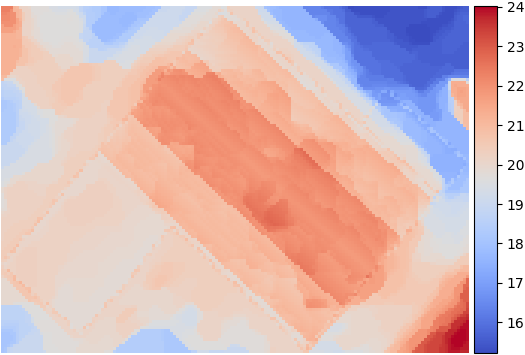
\includegraphics[width=3cm]{images/features/height/dsm-292034}};
        \path (dsm_1.south) node[anchor=north, text width=3cm, align=center, visible on=<1-2>] (dsm_legend) {\acrshort{acr::dsm}};

        \path (dsm_1.east) node[anchor=west, visible on=<2>] (minus_1) {\Large --};

		\path (minus_1.east) node[anchor=west, visible on=<2>] (model_1) {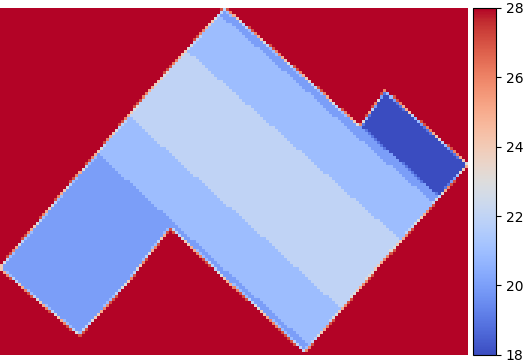
\includegraphics[width=3cm]{images/features/height/heightmap-292034}};
        \path (model_1.south) node[anchor=north, text width=3cm, align=center, visible on=<2>] (model_legend) {Model heights};

        \path (minus_1) node[visible on=<3>] (residual_1) {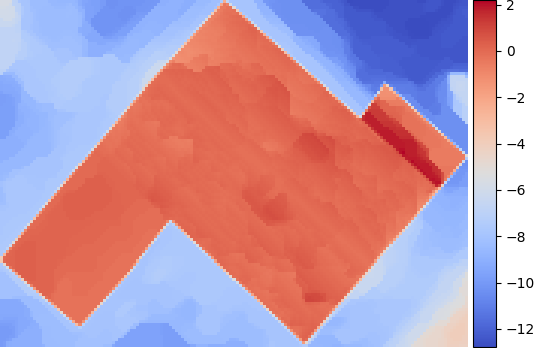
\includegraphics[width=3cm]{images/features/height/residual-292034}};
        \path (residual_1.south) node[anchor=north, text width=3cm, align=center, visible on=<3>] (residual_legend) {Residuals};

        \path (residual_1.west) node[anchor=east, visible on=<3>] (equals_1) {\Large =};

        \path (residual_legend.south) + (0, -.5) node[text width=4cm, align=center, visible on=<4>, anchor=north] (hist_legend) {Histogram};
        \path (hist_legend.north) + (-1.5, 1em) node[anchor=south] (hist_1) {};
        \begin{axis}[
            at={(hist_1)},
            width=4cm,
            area style,
            ymin=0,
            xmin=-14,
            xmax=14,
            xtick align=outside,
            ytick=\empty,
            xtick pos=left,
            ytick pos=left,
            visible on=<4>
        ]
            \addplot+[ybar interval,mark=no] plot coordinates {
                (-15, 0) 
                (-14, 0)
                (-13, 876)
                (-12, 366)
                (-11, 593)
                (-10, 675)
                (-9, 2231)
                (-8, 3623)
                (-7, 546)
                (-6, 159)
                (-5, 182)
                (-4, 70)
                (-3, 54)
                (-2, 123)
                (-1, 3815)
                (0, 4291)
                (1, 211)
                (2, 10)
                (3, 0)
                (4, 0)
                (5, 0)
                (6, 0)
                (7, 0)
                (8, 0)
            };
        \end{axis}
	\end{tikzpicture}
\end{document}
